\cleardoublepage
\chapter*{Einleitung}
\markboth{Einleitung}{Einleitung}
\addcontentsline{toc}{chapter}{Einleitung}
%text below here
Die Spielentwicklung als solches ist schon seit seiner Konzeption ein komplexes Feld, da es gutes Algebraisches Können verlangt. Das Model eines jeden Objekts, das dargestellt werden soll, besteht aus\cite{noauthor_polygon_2021}:


\begin{itemize}[noitemsep,topsep=0pt,parsep=0pt,partopsep=0pt]
	\item Vektoren
	\item Kanten
	\item Facetten
	\item Polygone
	\item Oberflächen 
\end{itemize}

\begin{figure}[h]
	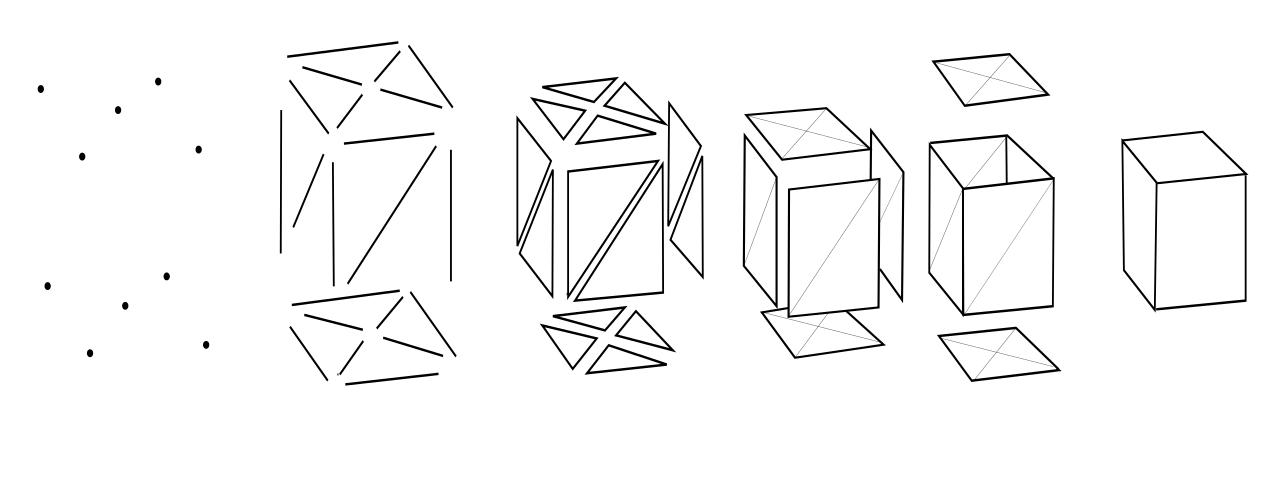
\includegraphics[width=13cm]{images/polygon_mesh}
	\caption{Visuelle Erläuterung\cite{diverse_polygon_2021} der oben gelisteten Daten, von Links nach Rechts}
	\label{fig:Visuelle Erläuterung nötiger Daten für ein 3D Quadrat}
\end{figure}

\newpage

Die Anzahl der einzelnen Daten variiert je nach Komplexität und Stil des Spiels stark. Als Beispiel\cite{astart_super_2017}: \\

Mario im Spiel \emph{Super Mario 64} aus 1996:
\begin{itemize}[noitemsep,topsep=0pt,parsep=0pt,partopsep=0pt]
	\item 406 Vektoren
	\item 752 Dreiseitige Polygone
	\item 752 Facetten\footnote{Die Anzahl Facetten sind meistens gleich wie die Anzahl Polygone, da man immer nur eine Seite sieht, d.h. die Seite des Polygons die im inneren eines Objektes ist wird nicht generiert}
\end{itemize}

Mario im Spiel \emph{Mario \& Sonic - Rio 2016 Olympic Games} aus 2016:
\begin{itemize}[noitemsep,topsep=0pt,parsep=0pt,partopsep=0pt]
	\item 406 5'606
	\item 10'656 Dreiseitige Polygone
	\item 20'656 Facetten
\end{itemize}

So kann  Diese genanten Vorgaben sind aber auch Grundlegende Bedingungen für das Entwickeln eines Spiels\footnote{Insofern man nicht rein Textbasierte Spiele entwickelt}. Dies führt dazu, das man eben diese Vorgaben abstrahieren kann und als Fertiglösung anderen zur Verfügung stellt. Die Herausgeber dieser Produkte ringen aber konstant um den Zahlenden Markt - so werden kontinuierlich neue Funktionalitäten hinzugefügt, oder bestehende Geändert. \\


